\documentclass[a4paper]{article}
\usepackage[margin=1in]{geometry}
\usepackage{fancyhdr}
\usepackage{caption}
\usepackage{tikz}
\usepackage{slashbox}
\pagestyle{fancy}
\setlength{\headheight}{30pt}
\lhead{Francisco Badilla - 2018135171\\Carlos Kruse - 2019046757}
\rhead{Proyecto II IC6400\\Modo ejemplo}
\begin{document}
\section*{Resultados del modo de ejemplo}
\subsection*{I. Descripción del problema}
Se tienen 6 llaves diferentes (A, B, C, D, E y F), cada una de las cuales tiene una probabilidad diferente de ser buscada. El objetivo es construir un \'arbol de b\'usqueda binario a partir de estas llaves, de forma que el tiempo de b\'usqueda promedio sea el menor posible. Para esto se emple\'o un algoritmo de programaci\'on din\'amica y un algoritmo greedy.

\subsection*{II. Datos del problema}
Los datos utilizados se resumen en la siguiente tabla:

\begin{table}[ht]
\centering
\begin{tabular}{r|l|l|l|l|l|l}
Llave & A & B & C & D & E & F  \\\hline
Probabilidad & 0.17 & 0.21 & 0.12 & 0.08 & 0.20 & 0.22
\end{tabular}
\label{datos}
\end{table}

\subsection*{III. Programación Dinámica}
A continuaci\'on se muestran las tablas generadas por el algoritmo de programaci\'on din\'amica para encontrar el \'arbol \'optimo. Adem\'as, se muestra el \'arbol resultante.

Tiempo de ejecución: 0.000004 segundos.
\begin{table}[ht]
\centering
\begin{tabular}{c|ccccccc}
\backslashbox{$i$}{$j$} & 0 & 1    & 2    & 3    & 4    & 5    & 6    \\ \hline
1 & 0.00 & 0.17 & 0.55 & 0.79 & 1.03 & 1.63 & 2.25 \\
2 & & 0.00 & 0.21 & 0.45 & 0.69 & 1.18 & 1.74 \\
3 & & & 0.00 & 0.12 & 0.28 & 0.68 & 1.12 \\
4 & & & & 0.00 & 0.08 & 0.36 & 0.80 \\
5 & & & & & 0.00 & 0.20 & 0.62 \\
6 & & & & & & 0.00 & 0.22 \\
7 & & & & & & & 0.00 \\

\end{tabular}
\caption{Matriz A generada por el algoritmo de programación din\'amica}
\label{A}
\end{table}

\begin{table}[ht]
\centering
\begin{tabular}{c|cccccc}
\backslashbox{$i$}{$j$} & 1    & 2    & 3    & 4    & 5    & 6    \\ \hline
1 & 1 & 2 & 2 & 2 & 2 & 5 \\
2 & & 2 & 2 & 2 & 3 & 5 \\
3 & & & 3 & 3 & 5 & 5 \\
4 & & & & 4 & 5 & 5 \\
5 & & & & & 5 & 6 \\
6 & & & & & & 6 \\

\end{tabular}
\caption{Matriz R generada por el algoritmo de programación din\'amica}
\label{R}
\end{table}

\begin{figure}[ht]
\centering
\begin{tikzpicture}[
every node/.style = {minimum width = 2.5em, draw, circle},
level/.style={sibling distance={3cm/max(1,#1)}, level distance=10mm}
]
\scriptsize
\node {E}
child {
node {B}
child {
node {A}
}
child {node {C}
child[missing]
child{
node {D}
}
}}
child {node {F}
};
\end{tikzpicture}
\caption{\'Arbol generado por el algoritmo de programación din\'amica}
\label{pd}
\end{figure}

\newpage
\subsection*{IV. Algoritmo Greedy}
A continuaci\'on se muestran la tabla R generada por el algoritmo greedy. Adem\'as, se muestra el \'arbol resultante.

Tiempo de ejecución: 0.000003 segundos.
\begin{table}[ht]
\centering
\begin{tabular}{c|cccccc}
\backslashbox{$i$}{$j$} & 1    & 2    & 3    & 4    & 5    & 6    \\ \hline
1 & 1 & 2 & 2 & 2 & 2 & 6 \\
2 & & 2 & 2 & 2 & 2 & 6 \\
3 & & & 3 & 3 & 5 & 6 \\
4 & & & & 4 & 5 & 6 \\
5 & & & & & 5 & 6 \\
6 & & & & & & 6 \\

\end{tabular}
\caption{Matriz R generada por el algoritmo greedy}
\label{Rg}
\end{table}

\begin{figure}[ht]
\centering
\begin{tikzpicture}[
every node/.style = {minimum width = 2.5em, draw, circle},
level/.style={sibling distance={6cm/max(1,#1)}, , level distance=10mm}
]
\scriptsize
\node {F}
child{
node {B}
child {
node {A}
}
child {node {E}
child{
node {C}
child[missing]
child{
node {D}
}
}
child[missing]
}}
child[missing]
;
\end{tikzpicture}
\caption{\'Arbol generado por el algoritmo greedy}
\label{greedy}
\end{figure}
\end{document}
